\chapter{State of the Art}
\label{ch:SOTA}

% "Introduction", kind of redundant with the summaries further down?
\section{What is blockchain?}
Blockchain is a decentralized, trustworthy distributed ledger on a peer to peer network that consists of a list of chronologically ordered blocks. Every block consists of a hash of a previous block and hence forming a chain. The first block in the blockchain is the genesis block and the block before a given block is called as its parent block \cite{blockchain}.

A block contains a header and body. The block header consists of 
\begin{itemize}
    \item Version: Specifies the block validation rules.
    \item Previous block hash: This is to ensure that the previous block cannot be changed, without changing the current block header.
    \item Timestamp: The current block creation time.
    \item Merkle root hash: The Merkle root is obtained from the hash values of all the transactions present in the block. This is to ensure that the transactions cannot be modified without changing the header.
    \item Nonce: A nonce is a 4 byte unique number that is used only once in the communication.
\end{itemize}

\begin{figure}[htbp]
 \centering
 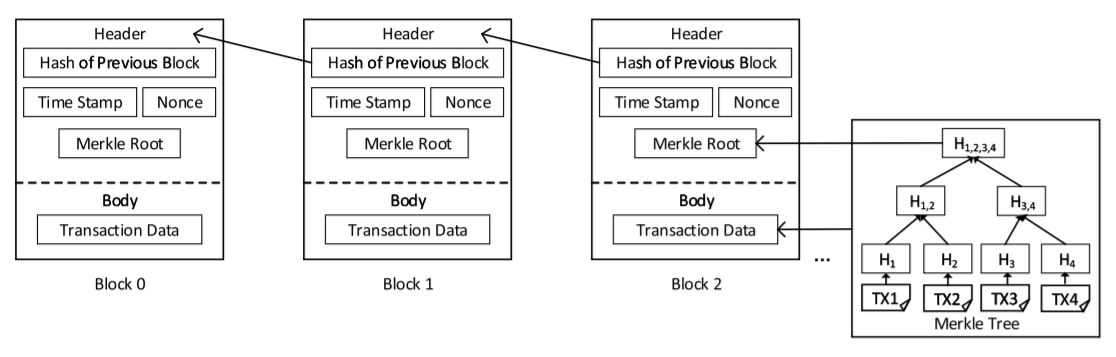
\includegraphics[width=1\textwidth, height=5cm]{gfx/figures/Block structure.JPG}
 \caption{Block Structure \cite{blockStructure}}
 \label{fig:chapter03:setup}
\end{figure}

The core components of blockchain architecture:
\begin{itemize}
    \item Node/Peer: A device (like a computer) present inside a blockchain network that has a copy of all the transactions.
    \item Transaction: It is the exchange of information between the two blockchain addresses.
    \item Block: It is used to keep a group of transactions that is distributed among all the nodes in the network.
    \item Chain: A series of blocks arranged in chronological order.
    \item Miners: Before adding any transactions to a new block node, selected nodes carry out the block verification.
    \item Consensus:  It is a mechanism through which all of the blockchain network's peers come to an agreement about any transaction in the blockchain.
\end{itemize}

\section{Evolution of blockchain}

The mainstream internet usage at the turn of the century aided the introduction of digital currency as an expansion of electronic cash systems. The following is a timeline of blockchain's growth.

\subsection{1991 - Blockchain Invention}
Scott Stornetta and Stuart Haber invented Blockchain. They created a cryptographically protected chain of blocks which would prevent anyone from tampering with document timestamps \cite{history}. 

\subsection{2008-2013 - Bitcoin Emergence}
Blockchain technology gained popularity due to Bitcoin in 2008, as it is the first application in the blockchain. Bitcoin was conceptualized by Satoshi Nakamoto. In 2009, Nakamoto published a white paper on Bitcoin. First Bitcoin was purchased for 10,000BTC in 2010. Bitcoin crosses \$1 billion in 2013.

\subsection{2013-2015 - Ethereum Development}
Ethereum was conceptualized by Vitalik Buterin. Ethereum has additional features like  smart contracts compared to Bitcoin. The development of  Ethereum has proven to be an important moment in the history of Blockchain.  Ethereum is used for cryptocurrencies and in many other decentralized applications because of smartcontracts.

 \subsection{2015 - Hyperledger}
Hyperledger was developed by Linux Foundation in 2015. It allows development of open-source blockchain. The different Hyperledger frameworks are Hyperledger Fabric, Hyperledger Iroha, Hyperledger Sawtooth, and Hyperledger Burrow \cite{hyperledgertypes}.

\subsection {2015 - Future}
Many cryptocurrencies and applications have been developed after the emergence of Bitcoin and Ethereum. Nowadays, Blockchain technology is used by various companies and organizations.

\section{Types of blockchain}

Blockchain is divided into four types, public, private, consortium and hybrid blockchains based on permission and assess.
\subsection{Public Blockchain}
It is a permissionless distributed technology. As the name suggests, anyone with the internet is allowed to access the public blockchain and participate in the transactions. Each peer in this network has their own copy of the ledger. Consensus mechanisms like \ac{PoW}, \ac{PoS}, etc., are required to reach consensus while adding new blocks and during verification of transactions. Public blockchains are fully decentralized because all the peers have equal authority, which in terms makes it secure as no one can have full control over the blockchain network. In turn,  ensuring data security helps in keeping the ledger immutable. Some examples are Bitcoin, Litecoin, and Ethereum.

Open and closed are used to tell who can read data in a blockchain. These two properties are used to describe blockchain.
\begin{itemize}
    \item Public and Open: This blockchain is accessible for everyone and data can be read by everyone. For example, cryptocurrencies like Bitcoin  and Ethereum.
    \item Public and Closed: The consumers can store confidential information and can restrict access for selected participants. In this blockchain, everyone can write in blockchain, but the reading rights are only held by selected entities. For example, Voting.
\end{itemize}


\subsection{Private Blockchain}
It is also known as permissioned blockchain. There are limitations on who can be part of the network and who can contribute to the transactions. A private blockchain is used by an organization or company for its internal usage. Private blockchains are centralized i.e, one organization has authority in the network. It provides transparency and security to the participants.
For example, Hyperledger Fabric.

\begin{itemize}
    \item Private and Open: Every contributor in the blockchain network can read the data. For example, Corporate income statements.
    
    \item Private and Closed: Only known participants can read and write in the blockchain network. For example, Tax returns, National Defense.
\end{itemize}

\subsection{Consortium Blockchain}
In this blockchain, more than one organization can manage the network, hence it is not fully centralized. It is used by organizations that need both public and private blockchain functionality. For example, Quorum and Hyperledger Fabric.


\subsection{Hybrid Blockchain}
 It is a mix of the private and public. In the blockchain, the peers determine who has access to which data. Some processes are kept private, while others are made public. On an open ledger, businesses can protect background transactions with business partners while still providing the product details to customers. For example, Dragonchain.

\section{Consensus algorithms}
All the peers have equal authority, hence it is difficult to reach consensus. Before Bitcoin, a lot of decentralized currency systems failed because when it came to reaching a consensus, they were unable to resolve the most important problem, i.e., Byzantine Generals Problem.\cite{blockchain}

\subsection{Byzantine generals problem}
The generals of various army battalions must choose whether to withdraw or assault. They must make a decision by sending messages by messengers and must reach an agreement. There's a possibility that some of the messengers and/or generals are traitors. These traitorous generals can change the message and send a malicious response, causing the loyal generals' plan to be disrupted.

\subsection{Consensus mechanisms}

The following are the few consensus mechanisms that can be used to address the issue of the Byzantine generals problem:

\subsubsection{Proof of Work} 
Bitcoin uses \ac{PoW} as the consensus mechanism. Miners “mine” a block to connect to the blockchain by solving cryptographic puzzles. This method requires a significant amount of energy and computation. The puzzles have been created in such a way that they are challenging and demanding on the system. When a miner completes the puzzle, they send their block for verification to the network. The method of determining whether a block belongs in the chain or not is extremely easy. A 51\% attack is a possible attack in the blockchain, in which a miner or a group of miners with more than 51\% of the computing power will prevent new blocks from being produced and establish false transaction records that benefit the attackers \cite{blockchain}.

\subsubsection{Proof of State}
It is a more energy-efficient version of \ac{PoW}. Nodes with the most stakes (for example, currency) are thought to be less likely to strike the network. The disadvantage here is the monopoly, when it comes to both technological and economic aspects of the scheme, the main stakeholder has full influence and authority.

\subsubsection{RAFT}
RAFT is a distributed crash fault tolerance consensus algorithm that ensures that the system can make a decision 
and process client requests in the event of a failure \cite{raft}. It is a consensus algorithm for handling a replicated log. 
Consensus in RAFT is reached through an elected leader. The server within a raft cluster is either a follower or a leader or a candidate. 
The leader is in charge of replicating logs to the followers.


\subsubsection{\ac{pBFT}}
Hyperledger fabric uses \ac{pBFT}. It is a realistic algorithm that tolerates Byzantine faults. \ac{pBFT} requires 3f+1 nodes in order to keep the system stable, where f is the maximum count of defective nodes the system can handle. As a result, approval from 2f+1 nodes is needed for the group of nodes to make any decision. Without performing complex mathematical computations (such as \ac{PoW}), \ac{pBFT} will achieve distributed consensus. Since they have been decided upon, the transactions do not need several confirmations. (For example, in Bitcoin's PoW , each node independently verifies all the transactions. Confirmations will take anywhere from 10 to 60 minutes depending on how many individuals have to confirm the new block).

\pagebreak

\section{Comparison between Hyperledger fabric and Ethereum}
\begin{table}[htbp]
\begin{center}

\begin{tabular}{ | m{3cm} | m{4.5cm}| m{4.5cm} | } 
\hline
& Hyperledger Fabric & Ethereum \\ 
\hline
Blockchain Type & Permissioned and Private & Permissionless and Private / Public\\ 
\hline
Objective & Suited for enterprises and B2B applications & Suited for B2C applications \\ 
\hline
Cryptocurrency & None & Ether \\ 
\hline
Smart contract language & JavaScript, GO and Java & Solidity \\ 
\hline
Consensus Mechanism & Pluggable consensus mechanism. Mining not required & \ac{PoW} consensus mechanism. Mining is required to reach the consensus.\\ 
\hline
Confidentiality & Confidential transactions & Transparent \\ 
\hline
\ac{tps} & > 2000 \ac{tps}  & $\approx$ 20 \ac{tps}  \\ 
\hline
\end{tabular}
\caption{Hyperledger fabric and Ethereum comparison}
\label{table:1}
    
\end{center}
\end{table}